%%%%%%%%%%%%%%%%%%%%%%%%%%%%%%%%%%%%%%%%%%%%%%%%%%%%%%%%%%%%%%%%%%%%%%%
% Based on IEEE the conference template available                     %
% at https://www.ieee.org/conferences/publishing/templates.html       %
% Adapted for the Data Science Lab course at Politecnico di Torino    %
% by Giuseppe Attanasio, Flavio Giobergia                             %
% 2020, DataBase and Data Mining Group                                %
%%%%%%%%%%%%%%%%%%%%%%%%%%%%%%%%%%%%%%%%%%%%%%%%%%%%%%%%%%%%%%%%%%%%%%%
\usepackage[T1]{fontenc}
\usepackage[utf8]{inputenc}
\documentclass[conference]{IEEEtran}
\usepackage{cite}
\usepackage{amsmath,amssymb,amsfonts}
\usepackage{placeins}
\usepackage{caption}
\usepackage{algorithmic}
\usepackage{graphicx}
\usepackage{textcomp}
\usepackage{xcolor}
\usepackage{float}
\begin{document}

\title{Report title}

\author{
\IEEEauthorblockN{Matteo Sisti}
\IEEEauthorblockA{\textit{Politecnico di Torino} \\
Student id: s362355 \\
matteo.sisti@studenti.polito.it}
\and
\IEEEauthorblockN{Beybin \c{C}i\c{c}ek}
\IEEEauthorblockA{\textit{Politecnico di Torino} \\
Student id: s351818 \\
beybin.cicek@studenti.polito.it}
}

\maketitle

\begin{abstract}
This project addresses a multi-class news article classification task on a real-world, HTML-heavy dataset characterized by noisy content, heterogeneous sources, and strong editorial regularities. The goal is to predict one of seven topical categories while optimizing macro-averaged F1 score. We first establish a linear baseline and introduce a two-stage classification strategy to separate near-deterministic cases from genuinely ambiguous documents. We then explore transformer-based architectures and analyze their stability across random seeds and input sequence lengths. Finally, we combine complementary models through ensemble strategies to improve robustness. Experimental results show that transformer-based models substantially outperform linear approaches, while ensembling yields further gains in overall performance.
\end{abstract}




\section{Problem Overview}

This project addresses a multi-class news article classification task, where
each document is assigned to one of seven topical categories. The dataset
consists of real-world online news articles in raw HTML format, characterized
by heterogeneous sources, noisy markup, incomplete metadata, and strong
editorial regularities. Performance is evaluated using macro-averaged F1 score
to ensure balanced behavior across classes.

A preliminary exploratory analysis is conducted to identify informative,
redundant, and structurally biased signals, guiding preprocessing and modeling
choices.

\paragraph{Temporal Metadata and Redundancy}
The \textit{timestamp} attribute contains a high proportion of missing values
(\textbf{34.7\%}) and exhibits coarse temporal granularity, with no clear
relationship between fine-grained temporal components and the target labels.
An auxiliary experiment shows that publication year can be predicted directly
from raw article text with approximately \textbf{64.0\%} accuracy, indicating
that temporal information is implicitly encoded in lexical and editorial
patterns. Consequently, explicit timestamp information is treated as redundant
and excluded.

\begin{center}
	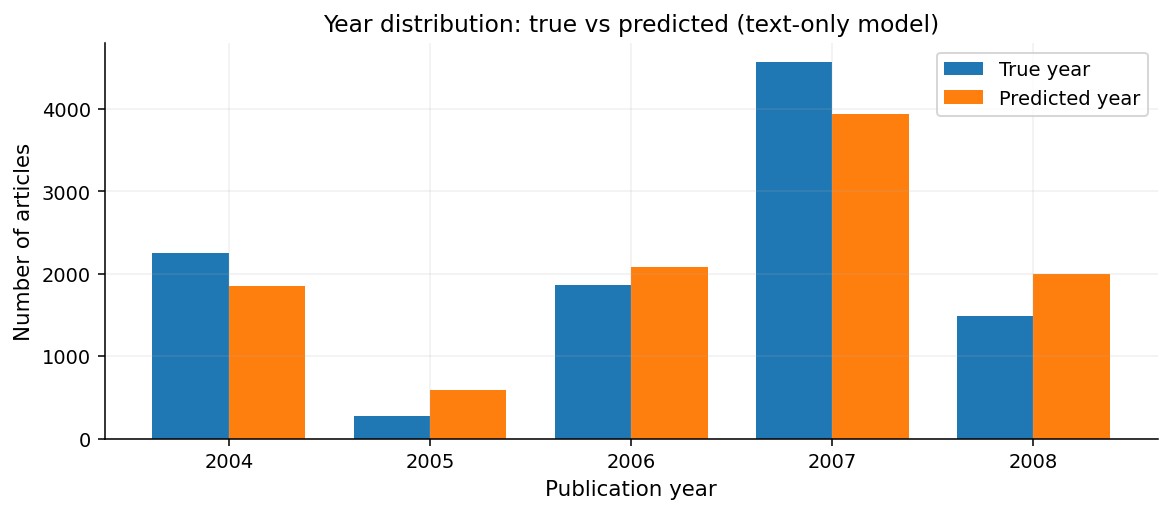
\includegraphics[width=\linewidth]{FIGURES/figure1_year_prediciton.png}
	\captionof{figure}{Distribution of publication years in the development set
	and corresponding predictions obtained from a text-only classifier,
	confirming that temporal information is implicitly encoded in the text.}
	\label{fig:year_prediction}
\end{center}

\paragraph{Non-informative Metadata}
The \textit{page\_rank} feature follows an approximately uniform distribution
and shows no meaningful correlation with the target labels. Its inclusion does
not provide measurable performance gains and is therefore discarded.

\paragraph{Structural Ambiguity}
The dataset contains duplicated or republished articles with identical content
assigned to different labels (\textbf{6.87\%} of the development set). This
introduces intrinsic ambiguity, defining an upper bound on achievable
performance and motivating the use of macro-averaged F1 score.

\paragraph{Editorial Bias and Source Informativeness}
A strong dependency exists between article source and target labels, reflecting
editorial specialization across publishers. One-hot encoding of source
information yields a strong linear baseline, revealing near-deterministic
editorial cues and motivating modeling strategies that separate structurally
deterministic from semantically ambiguous documents.

\textbf{[FIGURE 2 HERE: Source $\times$ Label heatmap]}

\paragraph{Implications}
Overall, the dataset combines noisy HTML-heavy text, redundant metadata, and
strong editorial regularities. These properties motivate a progressive modeling
approach that exploits high-confidence structural signals while reserving more
expressive models for genuinely ambiguous samples.



\section{Proposed approach}
The proposed approach combines structural and semantic modeling strategies to address dataset heterogeneity. Editorial patterns are captured through a Two-Stage classification pipeline, while Transformer-based models model high-level semantics. Final predictions are obtained by combining complementary models to improve robustness and generalization


\subsection{Preprocessing}
Preprocessing is lightweight, using concatenated and lowercased title and
article text. Linear and Two-Stage models incorporate simple numeric and
source features, while Transformer-based models rely exclusively on raw
text.

\subsection{Model selection}
\subsubsection{Editorial-Oriented Two-Stage Paradigm}

A linear TF--IDF baseline using word- and character-level n-grams, source
indicators, and simple numeric features is first evaluated. Despite extensive
hyperparameter exploration (Table~\ref{tab:baseline_hyperparams}), performance
saturates around a macro-averaged F1 score of $0.719$, indicating that a
single-stage linear formulation largely exhausts the available signal.

\begin{table}[H]
\centering
\caption{Optimal hyperparameter ranges for the linear TF--IDF baseline.}
\label{tab:baseline_hyperparams}
\begin{tabular}{lc}
\hline
\textbf{Hyperparameter} & \textbf{Selected value / range} \\
\hline
Word n-grams        & 2 \\
Character n-grams   & 5--7 \\
Regularization $C$  & 0.6--1.0 \\
Max document freq.  & 0.85--0.9 \\
\hline
\end{tabular}
\end{table}

Inspection of feature weights reveals that the strongest predictors are
editorial and structural cues, such as publisher identifiers, RSS markers,
and HTML fragments. Several of these tokens exhibit near-deterministic class
associations, as illustrated in Table~\ref{tab:low_entropy_tokens}.

\begin{table}[H]
\centering
\caption{Examples of high-support editorial tokens with near-zero conditional entropy.}
\label{tab:low_entropy_tokens}
\small
\resizebox{\linewidth}{!}{%
\begin{tabular}{lcccl}
\hline
\textbf{Token} & \textbf{Type} & \textbf{Support} & \textbf{Entropy} & \textbf{Dominant label} \\
\hline
\texttt{<h4>} & editorial & 628 & 0.00 & 2 \\
\texttt{</h4>} & editorial & 628 & 0.00 & 2 \\
\texttt{<p align="right">} & editorial & 311 & 0.00 & 2 \\
\texttt{<a href=...>} & editorial & 233 & 0.00 & 2 \\
\texttt{<img class="rss-ad">} & editorial & 196 & 0.00 & 2 \\
\texttt{<strong>} & editorial & 111 & 0.00 & 2 \\
\texttt{<cite>} & editorial & 40 & 0.00 & 2 \\
\texttt{<em>} & editorial & 57 & 0.47 & 2 \\
\hline
\end{tabular}}
\end{table}

To formalize this behavior, for a token $t$ and class label $Y$ we estimate the
empirical distribution $p(c \mid t)$ on the development set as the fraction of
documents containing $t$ that belong to class $c$. The conditional entropy is
defined as:
\[
H(Y \mid t) = - \sum_{c \in \mathcal{Y}} p(c \mid t)\log p(c \mid t).
\]
For a non-trivial subset of tokens, $H(Y \mid t)=0$, meaning that their presence
alone deterministically identifies the class in the development set.

Based on these observations, we adopt a Two-Stage classification paradigm. For
each token $t$, we compute:
\[
\text{purity}(t) = \max_{c \in \mathcal{Y}} p(c \mid t), \quad
\text{support}(t) = |\{x_i : t \in x_i\}|,
\]
where $\text{support}(t)$ denotes the number of development documents
containing $t$. Tokens satisfying purity and support thresholds $\tau_p$ and
$\tau_s$ are collected into a rule set:
\[
\mathcal{R} = \{t \in \mathcal{T} : \text{purity}(t) \ge \tau_p \;\wedge\;
\text{support}(t) \ge \tau_s\}.
\]

\paragraph{Stage 1: Deterministic Assignment}
If a document $x$ contains any token $t \in \mathcal{R}$, it is assigned the
corresponding dominant class:
\[
\hat{y}^{(1)}(x) = \arg\max_{c \in \mathcal{Y}} p(c \mid t).
\]

\paragraph{Stage 2: Probabilistic Classification}
All remaining documents are classified by a probabilistic model $f_\theta(x)$:
\[
\hat{y}^{(2)}(x) = \arg\max_{c \in \mathcal{Y}} f_\theta(x)_c.
\]

\paragraph{Unified Decision Rule}
\[
\hat{y}(x) =
\begin{cases}
\hat{y}^{(1)}(x), & \text{if } \exists\, t \in \mathcal{R} \text{ such that } t \in x, \\
\hat{y}^{(2)}(x), & \text{otherwise}.
\end{cases}
\]

This formulation explicitly separates deterministic editorial patterns from
semantically ambiguous instances, while reducing to a standard single-stage
classifier when no high-purity rules apply.

\subsubsection{Semantic-Oriented Transformer Models}

Transformer-based models are used to complement the editorial bias of the
Two-Stage classifier by modeling deeper semantic information. We fine-tune
RoBERTa and DeBERTa using only the concatenated title and article text, without
additional features. Predictions are treated independently and later combined
through ensemble strategies to exploit semantic complementarity.

\subsection{Hyperparameter Tuning}

Hyperparameter tuning is conducted to assess the sensitivity and
robustness of the proposed two-stage classifier, rather than to
aggressively maximize performance
\subsubsection{Two-Stage Rule Parameters}

We analyze the sensitivity of the Two-Stage classifier to the minimum rule
purity $\tau_p$, minimum rule support $\tau_s$, and the regularization
parameter $C$ of the Stage~2 classifier.

Figure~\ref{fig:purity_f1} shows that macro-averaged F1 increases monotonically
with the rule purity threshold, confirming that selecting highly pure patterns
consistently improves performance.

\begin{center}
	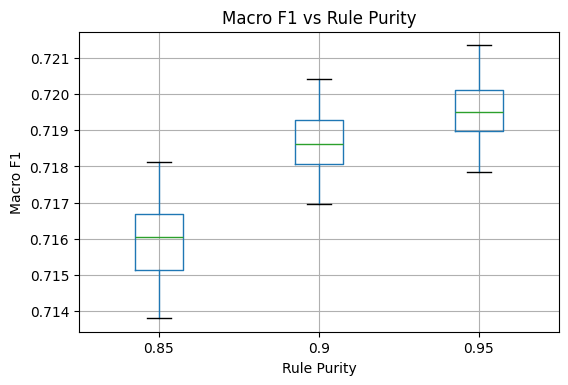
\includegraphics[width=0.7\linewidth]{FIGURES/F1_vs_RulePuriti.png}
	\captionof{figure}{Macro-averaged F1 score as a function of the rule purity threshold $\tau_p$.}
	\label{fig:purity_f1}
\end{center}

Figure~\ref{fig:support_f1} shows that performance remains largely stable across
a broad range of rule support thresholds, indicating limited sensitivity to
$\tau_s$ once sufficiently frequent patterns are retained.

\begin{center}
	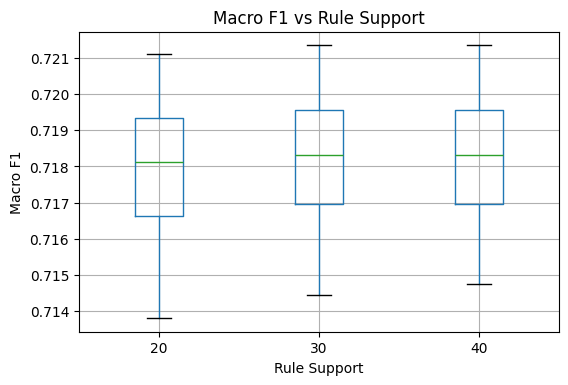
\includegraphics[width=0.7\linewidth]{FIGURES/F1_vs_RuleSupport.png}
	\captionof{figure}{Macro-averaged F1 score as a function of the rule support threshold $\tau_s$.}
	\label{fig:support_f1}
\end{center}

\paragraph{Linear Model Regularization}
The regularization parameter $C$ of the Stage~2 linear classifier is varied
across a wide range. As shown in Figure~\ref{fig:f1_vs_c}, macro-F1 remains
stable for moderate values of $C$, with only marginal degradation for larger
values.

\begin{center}
	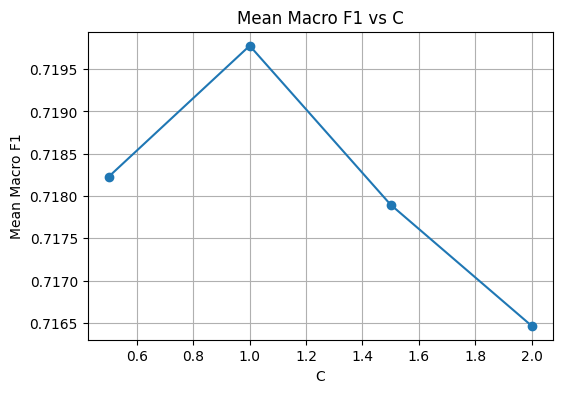
\includegraphics[width=0.7\linewidth]{FIGURES/macro_F1_vs_C.png}
	\captionof{figure}{Macro-averaged F1 score as a function of the regularization
	parameter $C$ for the Stage~2 classifier.}
	\label{fig:f1_vs_c}
\end{center}

\paragraph{Best Configurations}
Table~\ref{tab:best_twostage} reports the top-performing configurations on the
development set, together with the corresponding rule coverage.

\begin{table}[H]
\centering
\caption{Top-performing Two-Stage configurations on the development set.
Reported are the regularization parameter $C$, minimum rule purity $\tau_p$,
minimum rule support $\tau_s$, macro-averaged F1 score, and rule coverage.}
\label{tab:best_twostage}
\small
\begin{tabular}{ccccc}
\hline
\textbf{$C$} & \textbf{$\tau_p$} & \textbf{$\tau_s$} & \textbf{Macro F1} & \textbf{Coverage} \\
\hline
1.0  & 0.95 & 40 & 0.7214 & 0.156 \\
1.0  & 0.95 & 30 & 0.7214 & 0.162 \\
1.0  & 0.95 & 20 & 0.7211 & 0.172 \\
1.0  & 0.90 & 30 & 0.7204 & 0.189 \\
1.0  & 0.90 & 20 & 0.7202 & 0.202 \\
\hline
\end{tabular}
\end{table}

Overall, the results reveal a wide performance plateau across all considered
hyperparameters, indicating that the gains achieved by the Two-Stage approach
are driven by its structural decomposition rather than by fragile tuning.

\subsubsection{Transformer Fine-Tuning}

Transformer models are fine-tuned using a standardized and conservative
setup, consistent with common practices in document classification.
Given the large training set and the use of pre-trained language models,
training is limited to 2--4 epochs to ensure convergence while avoiding
overfitting and unnecessary computational overhead.
Learning rates are selected from widely adopted fine-tuning ranges to
guarantee stable optimization.

Batch size is fixed by hardware constraints and not treated as a tunable
parameter. To account for stochastic effects, each configuration is
evaluated across multiple random seeds (noseed, 42, 1337, 2024).

\paragraph{Intra-seed Stability}
Stability with respect to random initialization is assessed by measuring
prediction agreement across different seeds, since ground-truth labels
are unavailable for the evaluation set.
High agreement across all architectures indicates stable convergence and
limited sensitivity to stochastic optimization.

\begin{table}[h]
\centering
\caption{Intra-seed prediction agreement for transformer models.}
\label{tab:intra_seed_agreement}
\small
\begin{tabular}{lccc}
\hline
\textbf{Model} & \textbf{Mean Agreement} & \textbf{Std} & \textbf{\#Seeds} \\
\hline
DeBERTa-512  & 0.8968 & 0.0011 & 3 \\
DeBERTa-256  & 0.9073 & 0.0009 & 3 \\
RoBERTa-512  & 0.9114 & 0.0004 & 3 \\
RoBERTa-256  & 0.9112 & 0.0001 & 3 \\
\hline
\end{tabular}
\end{table}

\paragraph{Cross-Architecture Hard-Case Analysis}
To assess architectural complementarity, prediction overlap is analyzed
on a subset of hard cases, defined as samples consistently misclassified
by simpler models.
High cross-architecture agreement on these samples suggests that residual
errors are driven by intrinsic semantic ambiguity rather than
hyperparameter choices or model-specific artifacts.

\begin{figure}[t]
	\centering
	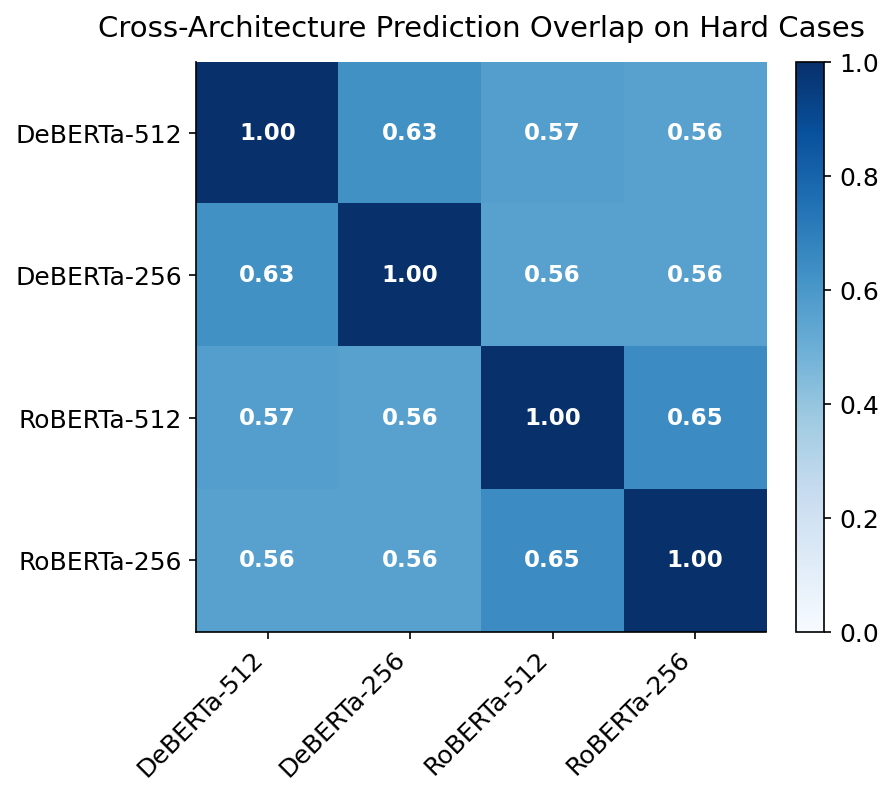
\includegraphics[width=0.75\linewidth]{FIGURES/overlap_hardcase}
	\caption{Cross-architecture prediction agreement on hard cases.
	Agreement is computed on samples with model disagreement, highlighting
	residual semantic ambiguity across transformer architectures.}
	\label{fig:cross_arch_overlap_hard}
\end{figure}

Overall, these analyses indicate that transformer fine-tuning operates in
a stable regime, with performance differences primarily determined by
architectural inductive biases rather than aggressive hyperparameter
optimization. Transformer models are therefore treated as robust semantic
baselines, whose complementarity is later exploited through ensemble
analysis.


\section{Results}
\subsection{Two-Stage Classification Results}

The Two-Stage classifier is evaluated over a wide range of rule-based and
linear-model hyperparameters. On the development set, macro-averaged F1
consistently stabilizes around $0.72$, indicating a broad near-optimal region
rather than sensitivity to a specific configuration.

Bayesian optimization is used to select a representative high-performing
setup, whose parameters and corresponding rule coverage are reported in
Table~\ref{tab:two_stage_params}. Comparable performance is achieved by
neighboring configurations, confirming robustness to hyperparameter choices.

On the evaluation set, the selected model achieves a macro-F1 of $0.731$.
The rule-based stage deterministically classifies approximately $16\%$ of
samples, while the remaining instances are handled by the probabilistic
classifier, highlighting that performance gains stem primarily from the
structural two-stage decomposition rather than aggressive tuning.

\begin{table}[H]
\centering
\caption{Selected hyperparameters from Bayesian Optimization and rule coverage for the Two-Stage classifier.}
\label{tab:two_stage_params}
\begin{tabular}{lc}
\hline
\textbf{Component} & \textbf{Value} \\
\hline
Min rule support          & 20 \\
Min rule purity           & 0.984 \\
Rule coverage (Eval)      & 0.164 \\
\hline
Word n-gram max           & 2 \\
Character n-gram max      & 5 \\
Min document frequency    & 3 \\
Max document frequency    & 0.908 \\
Regularization $C$        & 0.842 \\
\hline
\end{tabular}
\end{table}

\subsection{Transformer and Ensemble Results}

Transformer models are evaluated across RoBERTa and DeBERTa architectures
with input lengths of 256 and 512 tokens. On the development split, no-seed
models provide a consistent basis for comparison across configurations.

Across all settings, performance converges within three fine-tuning epochs,
with peak macro-F1 typically reached at the second or third epoch, indicating
stable and fast convergence. Multiple random initializations are trained to
reduce variance and support robust ensembling.

Final predictions are obtained via an ensemble selected based on
development-set performance and stability, and this ensemble is used for
submission.

\begin{table}[H]
\centering
\caption{Best no-seed transformer models on the development split. For each
configuration, the highest macro-F1 score and the corresponding training
epoch are reported.}
\label{tab:transformer_best_dev}
\begin{tabular}{lccc}
\hline
\textbf{Model} & \textbf{Max Len} & \textbf{Best Epoch} & \textbf{Macro-F1 (DEV)} \\
\hline
DeBERTa & 256 & 2 & 0.743 \\
DeBERTa & 512 & 2 & 0.747 \\
RoBERTa & 256 & 3 & 0.749 \\
RoBERTa & 512 & 3 & \textbf{0.756} \\
\hline
\end{tabular}
\end{table}

\section{Discussion}
Any relevant discussion goes here.

\bibliography{bibliography}
\bibliographystyle{ieeetr}

\end{document}
